\documentclass{beamer}
\mode<presentation>
\usepackage{amsmath}
\usepackage{amssymb}
%\usepackage{advdate}
\usepackage{adjustbox}
\usepackage{subcaption}
\usepackage{enumitem}
\usepackage{multicol}
\usepackage{listings}
\usepackage{xcolor}
\usepackage{comment}
 
\definecolor{codegreen}{rgb}{0,0.6,0}
\definecolor{codeblue}{rgb}{0.8,0.3,0.3}
\definecolor{codegray}{rgb}{0.5,0.5,0.5}
\definecolor{codepurple}{rgb}{0.58,0,0.82}
\definecolor{backcolour}{rgb}{0.99,0.99,0.99}
 
\lstdefinestyle{mystyle}{
    backgroundcolor=\color{backcolour},   
    commentstyle=\color{codegreen},
    keywordstyle=\color{codeblue},
    numberstyle=\tiny\color{codegray},
    stringstyle=\color{codepurple},
    basicstyle=\ttfamily\footnotesize,
    breakatwhitespace=false,         
    breaklines=true,                 
    captionpos=b,                    
    keepspaces=true,                 
    showspaces=false,                
    showstringspaces=false,
    showtabs=false,                  
    tabsize=5
}
 
\lstset{style=mystyle}

\usepackage{url}
\def\UrlBreaks{\do\/\do-}
\usetheme{Berlin}
\usecolortheme{whale}
\setbeamertemplate{footline}
{
  \leavevmode%
  \hbox{%
  \begin{beamercolorbox}[wd=\paperwidth,ht=2.5ex,dp=1ex,right]{author in head/foot}%
    \insertframenumber{} / \inserttotalframenumber\hspace*{2ex} 
  \end{beamercolorbox}}%
  \vskip0pt%
}
\setbeamertemplate{navigation symbols}{}

\providecommand{\nCr}[2]{\,^{#1}C_{#2}} % nCr
\providecommand{\nPr}[2]{\,^{#1}P_{#2}} % nPr
\providecommand{\mbf}{\mathbf}
\providecommand{\pr}[1]{\ensuremath{\Pr\left(#1\right)}}
\providecommand{\qfunc}[1]{\ensuremath{Q\left(#1\right)}}
\providecommand{\sbrak}[1]{\ensuremath{{}\left[#1\right]}}
\providecommand{\lsbrak}[1]{\ensuremath{{}\left[#1\right.}}
\providecommand{\rsbrak}[1]{\ensuremath{{}\left.#1\right]}}
\providecommand{\brak}[1]{\ensuremath{\left(#1\right)}}
\providecommand{\lbrak}[1]{\ensuremath{\left(#1\right.}}
\providecommand{\rbrak}[1]{\ensuremath{\left.#1\right)}}
\providecommand{\cbrak}[1]{\ensuremath{\left\{#1\right\}}}
\providecommand{\lcbrak}[1]{\ensuremath{\left\{#1\right.}}
\providecommand{\rcbrak}[1]{\ensuremath{\left.#1\right\}}}
\theoremstyle{remark}
\newtheorem{rem}{Remark}
\newcommand{\sgn}{\mathop{\mathrm{sgn}}}
\providecommand{\abs}[1]{\left\vert#1\right\vert}
\providecommand{\res}[1]{\Res\displaylimits_{#1}} 
\providecommand{\norm}[1]{\lVert#1\rVert}
\providecommand{\mtx}[1]{\mathbf{#1}}
\providecommand{\mean}[1]{E\left[ #1 \right]}
\providecommand{\fourier}{\overset{\mathcal{F}}{ \rightleftharpoons}}
%\providecommand{\hilbert}{\overset{\mathcal{H}}{ \rightleftharpoons}}
\providecommand{\system}{\overset{\mathcal{H}}{ \longleftrightarrow}}
	%\newcommand{\solution}[2]{\textbf{Solution:}{#1}}
%\newcommand{\solution}{\noindent \textbf{Solution: }}
\providecommand{\dec}[2]{\ensuremath{\overset{#1}{\underset{#2}{\gtrless}}}}
\newcommand{\myvec}[1]{\ensuremath{\begin{pmatrix}#1\end{pmatrix}}}
\let\vec\mathbf

\lstset{
%language=C,
frame=single, 
breaklines=true,
columns=fullflexible
}

\numberwithin{equation}{section}

\title{Voice Recognition}
\author{ Rohith Ingilela \\ EE19BTECH11005 \\ Dept. of Electrical Engineering \\ IIT Hyderabad}

\date{\today} 
\begin{document}

\begin{frame}
\titlepage
\end{frame}
\begin{frame}
\tableofcontents
\end{frame}
\section{Data Augmentation}
\begin{frame}{Data Augmentation}
\begin{description}[font=$\bullet$~\normalfont\scshape\color{red!50!black}]
\item [] Data augmentation is a strategy that increase the diversity of data available for training models, without actually collecting new data.
\item [] Data augmentation for audio involves noise injection, shifting time, changing pitch and speed. 
\item [] \textbf{Zero Padding} is done to ensure all the data is of same length.
\item [] In \textbf{Zero Padding}, we create an empty array with desired size used for training and add augmented audio data to it.
\end{description}
\end{frame}
\section{Feature extraction}
\begin{frame}{Feature extraction}
\textbf{Mel Frequency Cepstral Coefficents (MFCCs)} relates perceived frequency, or pitch of a pure tone to its actual measured frequency. The Mel scale coefficients are given by:
\begin{equation*}
     Mel(f) = 1125\ln({1 + \frac{f}{700}})
 \end{equation*}
 On our dataset we get mfcc data of shape [49x39] i.e, 49 time steps with 39 features each.
\end{frame}
\section{Recurrent Neural Networks}
\begin{frame}{Recurrent Neural Networks}
\textbf{Recurrent Neural Network(RNN)} are a type of Neural Network where the output from previous are fed as input to the current step. \\ The main and most important feature of RNN is Hidden state, which remembers some information about a sequence. \\
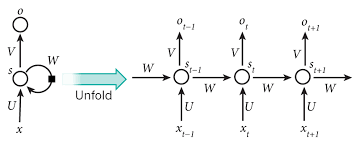
\includegraphics[width=0.5\columnwidth]{./figs/rnn_img.png} \\
We use a non linear activation function like tanh or ReLU to compute output of each node. \\
\end{frame}
\section{LSTM}
\begin{frame}{LSTM}
Long Short Term Memory networks(LSTM) – are a special kind of RNN, capable of learning long-term dependencies.\\
%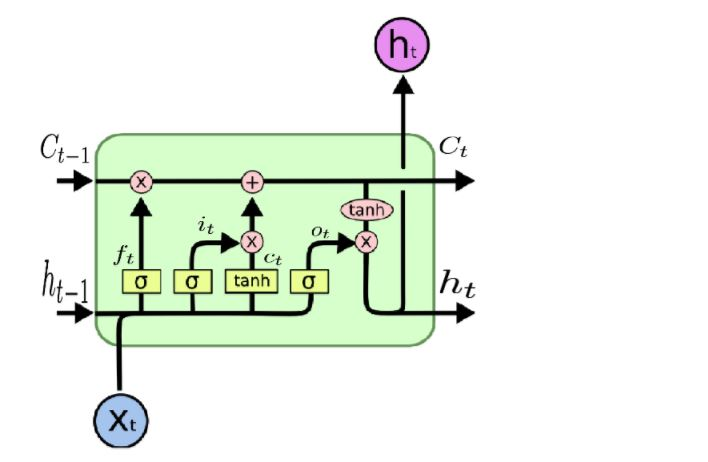
\includegraphics[width=0.5\columnwidth]{./figs/lstm_img.jpg} \\
LSTM layer can be used to exploit the sequential nature of sound files. \\
In LSTM we have a special gate known as forget gate, which makes the output from non related nodes non significant. \\ So, the long range memories exist without the gradients vanishing.
\end{frame}
\begin{frame}{}
    \textbf{Loss function : } Categorical Cross Entropy \\
    The input to the function is predicted probability and a one hot vector \\
It computes the loss by summing over the expression -ylog(p). \\
This is summed over a batch and the final loss is given
    \begin{equation*}
    %\sum_{n =1}^{T} E(y_t,\hat{y_t})
        E = -\sum_{i =1}^{c}y_i log(\hat{y_i})
    \end{equation*}
    \textbf{Stochastic Gradient decent : } It is the optimizer used for learning. \\ It tries to minimize the loss function by updating parameters through back propagation based on values of $\frac{\partial E}{\partial y}$.
\end{frame}
\end{document}